\chapter{نظرية  البيان}

\section{تعاريف و امثلة}

\begin{definition}
	البيان $G$ عبارة عن ثنائي مرتب $(V,E)$ حيث $V$ هي مجموعة غير خالية منتهية من العقد \en{Vertcies} و $E$ هي مجموعة الاسهم \en{Edges}.
\end{definition}

\begin{example}
	ليكن لدينا مجموعة من المطارات في دولة ما. بعض تلك المطارات يرتبط برحلات مباشرة مع مطارات اخرى من نفس البلد او مع بلدان اخرى و البعض الاخر يرتبط مع باقي المطارات.
	
\begin{figure}[H]
	\centering
		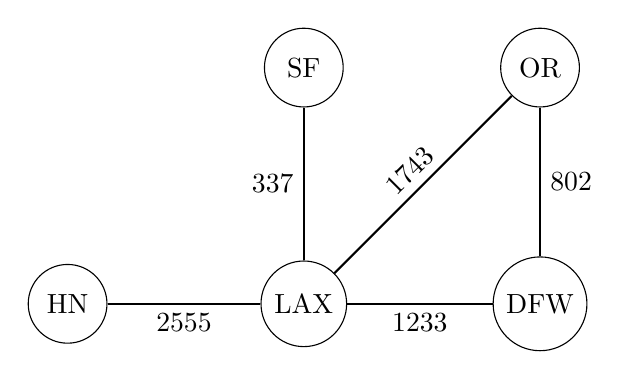
\begin{tikzpicture}
		% Node A
		\node[circle, draw, minimum size=1cm] (HN) at (0, 0) {HN};
		% Node B
		\node[circle, draw, minimum size=1cm] (LAX) at (3, 0) {LAX};
		% Node C
		\node[circle, draw, minimum size=1cm] (SF) at (3, 3) {SF};
		% Node D
		\node[circle, draw, minimum size=1cm] (OR) at (6, 3) {OR};
		% Node E
		\node[circle, draw, minimum size=1cm] (DFW) at (6, 0) {DFW};
		
		% Edges between nodes
		\draw[thick]  (HN) -- (LAX) node[midway, below] {2555};  
		\draw[thick] (SF) -- (LAX) node[midway, left]{337};  
		\draw[thick] (LAX) -- (OR) node[midway, above, sloped]{1743};  
		\draw[thick] (OR) -- (DFW) node[midway, right]{802};  
		\draw[thick] (LAX) -- (DFW) node[midway, below]{1233};
	\end{tikzpicture}
\end{figure}
	
	في الشكل اعلاه عبرنا عن كل مطار بنقطة و اذا كان مطاران مرتبطان برحلة مباشرة نمثلها بخط و على الخط يمكن ان نضع المسافة بين المطارين.
\end{example}

\noindent
\textbf{ملاحظات}
\begin{enumerate}
	\item كل سهم له عقدة او عقدتين مرتبطتين تسمى أطراف السهم \en{Endpoints}.
	\item يسمى السهم الذي له عقدة واحدة مرتبطة به بالحلقة \en{Loop}.
	\item تسمى الاسهم التي تتشارك بنفس النهايات بالاسهم المتوازية \en{Parallel}.
	\item تسمى العقدتين المرتبطتين بالسهم على انهما متجاورتين \en{Adjacent}.
	\item  تسمى العقدة التي ليس لها اسهم واردة بالمعزولة \en{Isolated}.
\end{enumerate}

\begin{example}
	ليكن لدينا البيان
\begin{figure}[H]
\centering
\begin{tikzpicture}[->, thick]
\node[fill=black, circle, draw, inner sep=2pt, label={left: $v_1$}] (v1) at (0,0) {};
\node[fill=black, circle, draw, inner sep=2pt, label={left: $v_2$}] (v2) at (0,3) {};
\node[fill=black, circle, draw, inner sep=2pt, label={right: $v_3$}] (v3) at (3,3) {};
\node[fill=black, circle, draw, inner sep=2pt, label={right: $v_4$}] (v4) at (3,0) {};
\node[fill=black, circle, draw, inner sep=2pt, label={right: $v_5$}] (v5) at (5,2) {};
\node[fill=black, circle, draw, inner sep=2pt, label={right: $v_6$}] (v6) at (7,0) {};
\node[fill=black, circle, draw, inner sep=2pt, label={right: $v_7$}] (v7) at (10,2) {};

	
	\path (v1) edge node[midway, above] {$e_1$} (v4);
	\path (v4) edge [loop below] node[midway, below] {$e_5$} (v4);
	\path (v3) edge node[midway, right] {$e_4$} (v4);
	\draw[->, thick] (v2) .. controls (2,2) .. (v3) node[midway, below]{$e_2$};
	\draw[->, thick] (v3) .. controls (2,4) .. (v2) node[midway, above]{$e_3$};
	\path (v6) edge node[midway,above, sloped] {$e_6$} (v7);
\end{tikzpicture}
\end{figure}
في الشكل اعلاه السهم $e_5$ مثال على الحلقة و $e_2,e_3$ أسهم متوازية و العقدة $v_5$ مثال على العقدة المعزولة و العقدتان $v_6,v_7$ مثال على العقد المتجاورة.
\end{example}

\begin{example}
	ليكن لدينا البيان التالي
	\begin{figure}[H]
		\centering
		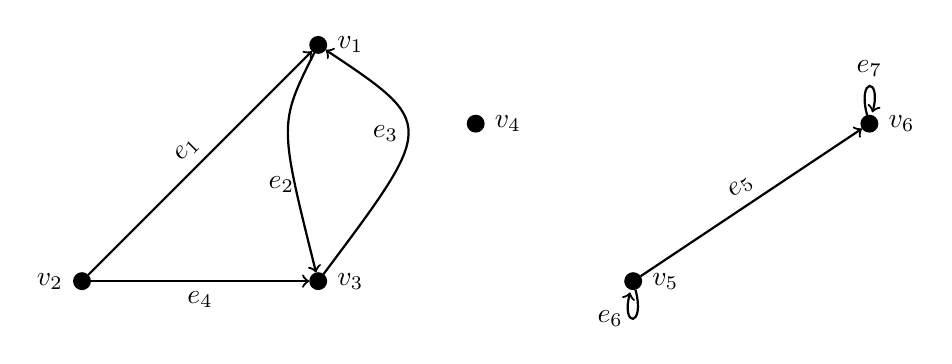
\begin{tikzpicture}[->, thick]
\node[fill=black, circle, draw, inner sep=2pt, label={left: $v_2$}] (v2) at (0,0) {};
\node[fill=black, circle, draw, inner sep=2pt, label={right: $v_1$}] (v1) at (3,3) {};
\node[fill=black, circle, draw, inner sep=2pt, label={right: $v_3$}] (v3) at (3,0) {};
\node[fill=black, circle, draw, inner sep=2pt, label={right: $v_4$}] (v4) at (5,2) {};
\node[fill=black, circle, draw, inner sep=2pt, label={right: $v_5$}] (v5) at (7,0) {};
\node[fill=black, circle, draw, inner sep=2pt, label={right: $v_6$}] (v6) at (10,2) {};

           
           \path (v2) edge node[midway, below]{$e_4$} (v3);
           \path (v2) edge node[midway, sloped, above]{$e_1$} (v1);
           \path (v5) edge node[midway, sloped, above]{$e_5$} (v6);
           
	      \draw[->, thick] (v1) .. controls (2.5,2) .. (v3) node[shift={(-5pt,35pt)},left]{$e_2$};
	      \draw[->, thick] (v3) .. controls (4.5,2) .. (v1) node[midway, left]{$e_3$};
	      	\path (v5) edge [loop below] node[midway, left] {$e_6$} (v5);
	        \path (v6) edge [loop above] node[midway, above] {$e_7$} (v6);		\end{tikzpicture}
	\end{figure}
	\noindent
	مجموعة العقد $\{v_1,v_2,v_3,v_4,v_5,v_6\}=$\\
		مجموعة الأسهم $\{e_1,e_2,e_3,e_4,e_5,e_6\}=$\\
		\begin{table}[H]
			\centering
			\begin{tabular}{|c|c|}
				\hline
				السهم & نهايتي السهم\\
				\hline
				$e_1$ & $\{v_1, v_2\}$\\
				$e_2$ & $\{v_1, v_3\}$\\
				$e_3$ & $\{v_1, v_3\}$\\
				$e_4$ & $\{v_2, v_3\}$\\
				$e_5$ & $\{v_5, v_6\}$\\
				$e_6$ & $v_5$\\
				$e_7$ & $v_6$\\
				\hline
			\end{tabular}
		\end{table} 
		\noindent
نلاحظ أن $e_6,e_7$ هي حلقات و $v_4$ عقدة معزولة
\end{example}

\noindent
\textbf{ملاحظة}\\
\noindent
يمكن لمجموعة العقد $V$ للبيان $G$ أن تكون غير منتهية $|V|=\infty$ نسمي البيان الذي له عدد غير منته من العقد أو عدد غير منته من الاسهم بالبيان غير المنتهي \en{Infinite Graph}.

\section{خواص البيانات}

\subsection{البيان البسيط}
ليكن $G$ بيان، يسمى $G$ بيان بسيط اذا كان لا يحتوي أية حلقات أو أسهماً متوازية. في البيان البسيط نرمز للسهم المحدد بالطرفين $v,w$ بــــــ $\{v,w\}$
\begin{example}
	لتكن $V=\{u,v,wx\}$ مجموعة عقد و لدينا سهمان احدهما $\{u,v\}$، عدد الاسهم الممكنة من اربعة عقد هي 6 اسهم كما يلي
	\[
	\{u,v\}, \{u,w\}, \{u,x\}, \{v,w\}, \{v,x\}, \{w,x\}
	\]
	واحد منها هو $\{u,v\}$ بالتالي السهم الثاني يمكن ان يكون واحد من الاسهم  الخمسة المتبقية
	\begin{figure}[H]
		\centering
		\begin{subfigure}{0.3\textwidth}
			\centering
			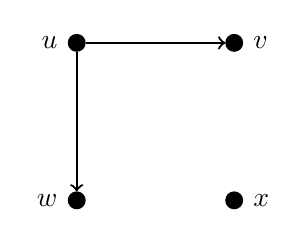
\begin{tikzpicture}[->, thick]
	 \node[fill=black, circle, draw, inner sep=2pt, label={left: $u$}] (u) at (0,0) {};
	 \node[fill=black, circle, draw, inner sep=2pt, label={right: $v$}] (v) at (2,0) {};
	 \node[fill=black, circle, draw, inner sep=2pt, label={left: $w$}] (w) at (0,-2) {};
	 \node[fill=black, circle, draw, inner sep=2pt, label={right: $x$}] (x) at (2,-2) {};
	 
	            
	            \path (u) edge (v);
	             \path (u) edge (w);
			\end{tikzpicture}
		\end{subfigure}
		\begin{subfigure}{0.3\textwidth}
			\centering
			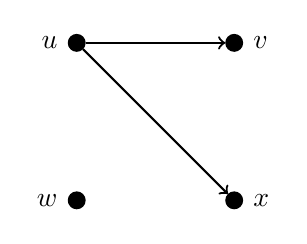
\begin{tikzpicture}[->, thick]
			\node[fill=black, circle, draw, inner sep=2pt, label={left: $u$}] (u) at (0,0) {};
			\node[fill=black, circle, draw, inner sep=2pt, label={right: $v$}] (v) at (2,0) {};
			\node[fill=black, circle, draw, inner sep=2pt, label={left: $w$}] (w) at (0,-2) {};
			\node[fill=black, circle, draw, inner sep=2pt, label={right: $x$}] (x) at (2,-2) {};
			
				
				 \path (u) edge (v);
				  \path (u) edge (x);
			\end{tikzpicture}
		\end{subfigure}
		\begin{subfigure}{0.3\textwidth}
			\centering
			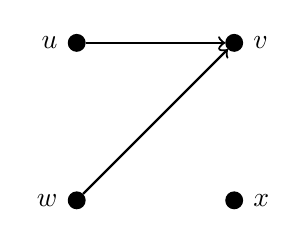
\begin{tikzpicture}[->, thick]
			\node[fill=black, circle, draw, inner sep=2pt, label={left: $u$}] (u) at (0,0) {};
			\node[fill=black, circle, draw, inner sep=2pt, label={right: $v$}] (v) at (2,0) {};
			\node[fill=black, circle, draw, inner sep=2pt, label={left: $w$}] (w) at (0,-2) {};
			\node[fill=black, circle, draw, inner sep=2pt, label={right: $x$}] (x) at (2,-2) {};
			
				
				 \path (u) edge (v);
				  \path (w) edge (v);
			\end{tikzpicture}
		\end{subfigure}
	\end{figure}
	
\begin{figure}[H]	
	\centering
		\begin{subfigure}{0.3\textwidth}
		\centering
		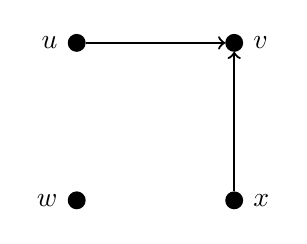
\begin{tikzpicture}[->, thick]
		\node[fill=black, circle, draw, inner sep=2pt, label={left: $u$}] (u) at (0,0) {};
		\node[fill=black, circle, draw, inner sep=2pt, label={right: $v$}] (v) at (2,0) {};
		\node[fill=black, circle, draw, inner sep=2pt, label={left: $w$}] (w) at (0,-2) {};
		\node[fill=black, circle, draw, inner sep=2pt, label={right: $x$}] (x) at (2,-2) {};
		
			
			 \path (u) edge (v);
			  \path (x) edge (v);
		\end{tikzpicture}
	\end{subfigure}
	\begin{subfigure}{0.3\textwidth}
		\centering
		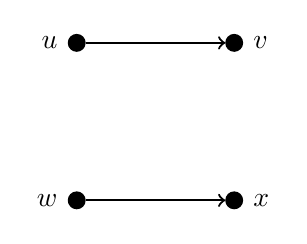
\begin{tikzpicture}[->, thick]
\node[fill=black, circle, draw, inner sep=2pt, label={left: $u$}] (u) at (0,0) {};
\node[fill=black, circle, draw, inner sep=2pt, label={right: $v$}] (v) at (2,0) {};
\node[fill=black, circle, draw, inner sep=2pt, label={left: $w$}] (w) at (0,-2) {};
\node[fill=black, circle, draw, inner sep=2pt, label={right: $x$}] (x) at (2,-2) {};

			
			 \path (u) edge (v);
			  \path (w) edge (x);
		\end{tikzpicture}
	\end{subfigure}
	\end{figure}
\end{example}

\subsection{البيان الموجه}
البيان $G=(V,E)$ حيث $V$ مجموعة غير خالية من العقد و $E$ هي مجموعة الاسهم الموجهة، حيث كل سهم يرتبط بزوج مرتب من العقد ندعوها طرفي السهم .Endpoints
\begin{example}
	في البيان الموجه اذا وجد سهم من $v$ الى $w$ فليس من الضروري ان يوجد سهم من $w$ الى $v$ اي لدينا زوج مرتب $\{v,w\}$ بمعنى 
	$\{v,w\} \neq \{w,v\}$
	نسمي العقدة $v$ بالذيل tail و $w$ بالرأس head
\end{example}

\subsection{درجة العقدة}
هي عدد الاسهم التي تصل الى العقدة، و اذا كان السهم حلقة نعيده مرتين. و نرمز لها بالرمز $\deg(v)$

\subsection{الدرجة الكلية}
هي مجموع درجات العقد التي يتألف منها 
\[
\deg(G) = \sum_{v\in V}^{} \deg(v)
\]

\begin{example}
	ليكن لدينا البيان
	\begin{figure}[H]
		\centering
		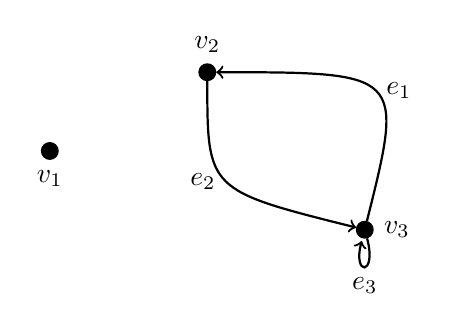
\begin{tikzpicture}[->, thick]
			\node[fill=black, circle, draw, inner sep=2pt, label={below: $v_1$}] (v1) at (0,1) {};
			\node[fill=black, circle, draw, inner sep=2pt, label={above: $v_2$}] (v2) at (2,2) {};
			\node[fill=black, circle, draw, inner sep=2pt, label={right: $v_3$}] (v3) at (4,0) {};
			
				
				\path (v3) edge [loop below] node[midway, below] {$e_3$} (v3);
				\draw[->, thick] (v2) .. controls (2,0.5) .. (v3) node[midway, left]{$e_2$};
				\draw[->, thick] (v3) .. controls (4.5,2) .. (v2) node[midway, right]{$e_1$};
		\end{tikzpicture}
	\end{figure}
	\[
	\Rightarrow \deg(v_1) = 0 , \quad \deg(v_2) = 2, \quad \deg(v_3) = 4
	\]
	\[
	\Rightarrow \deg(G) = 0 + 2 + 4 = 6
	\]
\end{example}

\begin{theorem}
	ليكن في البيان $G=(V,E)$ غير الموجه $n$ من الاسهم. يكون لدينا 
	\[
	\sum_{v\in V}^{} \deg(v) = 2n
	\] 
\end{theorem}

\begin{corollary}
	الدرجة الكلية لبيان هي عدد زوجي.
\end{corollary}

\begin{theorem}
	في البيان غير الموجه يوجد عدد زوجي من العقد التي درجتها عدد فردي.
\end{theorem}
\noindent
\textbf{الدرجة الواردة \en{in-degree}:} لعقدة $v$ في بيان موجه هي عدد الاسهم التي تصل هذه العقدة و نرمز لها بالرمز $\deg_-(v)$\\[10pt]
\textbf{الدرجة الصادرة (الخارجة) \en{out-degree}:} لعقدة $v$ في بيان موجه هي عدد الاسهم التي تخرج من هذه العقدة و نرمز لها بالرمز $\deg_+(v)$

\begin{theorem} 
	ليكن في البيان $G=(V,E)$ الموجه $n$ من الاسهم يكون لدينا
	\[
	\sum_{v\in V}^{} \deg_-(v) = \sum_{v\in V}^{} \deg_+(v) = n 
	\]
\end{theorem}

\section{انواع خاصة من البيانات}

\subsection{البيانات التامة \en{Complete Graphs}}
هي عبارة عن بيانات بسيطة بــ $n$ من العقد بحيث انها تحتوي على سهم واحد بين كل زوج من العقد المختلفة. و نرمز لها بــ $K_n$ كما في الشكل التالي:

\begin{english}
	\begin{figure}[H]
	\centering
	\begin{subfigure}{0.3\textwidth}
					\centering
		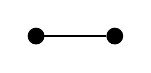
\begin{tikzpicture}
		    \node[circle, draw, fill=black, inner sep=2pt] (v1) at (0,0) {};
		    \node[circle, draw, fill=black, inner sep=2pt] (v4) at (1,0) {};
		    
		    \draw[thick] (v1) -- (v4);
		\end{tikzpicture}
		\caption{$K_2$}
	\end{subfigure}
\hfill
	\begin{subfigure}{0.3\textwidth}
		\centering
	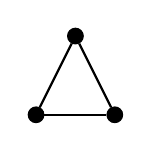
\begin{tikzpicture}
		\node[circle, draw, fill=black, inner sep=2pt] (v1) at (0,0) {};
		\node[circle, draw, fill=black, inner sep=2pt] (v3) at (0.5,1) {};
		\node[circle, draw, fill=black, inner sep=2pt] (v4) at (1,0) {};
		
		\draw[thick] (v1) -- (v3);
		\draw[thick] (v1) -- (v4);
		\draw[thick] (v3) -- (v4);
	\end{tikzpicture}
	\caption{$K_3$}
\end{subfigure}
\hfill
	\begin{subfigure}{0.3\textwidth}
					\centering
			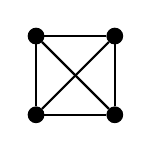
\begin{tikzpicture}
			\node[circle, draw, fill=black, inner sep=2pt] (v1) at (0,0) {};
			\node[circle, draw, fill=black, inner sep=2pt] (v2) at (0,1) {};
			\node[circle, draw, fill=black, inner sep=2pt] (v3) at (1,1) {};
			\node[circle, draw, fill=black, inner sep=2pt] (v4) at (1,0) {};
			
			\draw[thick] (v1) -- (v2);
			\draw[thick] (v1) -- (v3);
			\draw[thick] (v1) -- (v4);
			\draw[thick] (v2) -- (v3);
			\draw[thick] (v2) -- (v4);
			\draw[thick] (v3) -- (v4);
		\end{tikzpicture}
		\caption{$K_4$}
	\end{subfigure}
	\hfill
	\begin{subfigure}{0.3\textwidth}
		\centering
		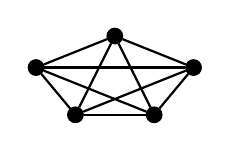
\begin{tikzpicture}
			% Define the vertices using the provided coordinates
			\node[circle, draw, fill=black, inner sep=2pt] (v1) at (0,0) {};
			\node[circle, draw, fill=black, inner sep=2pt] (v2) at (1,0) {};
			\node[circle, draw, fill=black, inner sep=2pt] (v3) at (0.5,1) {};
			\node[circle, draw, fill=black, inner sep=2pt] (v4) at (-0.5,0.6) {};
			\node[circle, draw, fill=black, inner sep=2pt] (v5) at (1.5,0.6) {};
			
			% Draw the edges between all pairs of vertices (complete graph K_5)
			\draw[thick] (v1) -- (v2);
			\draw[thick] (v1) -- (v3);
			\draw[thick] (v1) -- (v4);
			\draw[thick] (v1) -- (v5);
			\draw[thick] (v2) -- (v3);
			\draw[thick] (v2) -- (v4);
			\draw[thick] (v2) -- (v5);
			\draw[thick] (v3) -- (v4);
			\draw[thick] (v3) -- (v5);
			\draw[thick] (v4) -- (v5);
		\end{tikzpicture}
		\caption{$K_5$}
	\end{subfigure}
\end{figure}
\end{english}

\subsection{البيانات الدائرية \en{Cycles}}
هي عبارة عن بيانات بسيطة بــ $n$ من العقد حيث $(n\geq3)$ $v_1, v_2, \dots, v_n$ و $n-1$ من الاسهم 
$\{v_1, v_2\}, \{v_2, v_3\}, \dots, \{v_{n-1}, v_n\}$
ونرمز لها بالرمز $C_n$ كما في الشكل التالي
\begin{english}
	\begin{figure}[H]
		\centering
		\begin{subfigure}{0.3\textwidth}
			\centering
			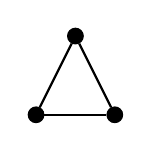
\begin{tikzpicture}
				\node[circle, draw, fill=black, inner sep=2pt] (v1) at (0,0) {};
				\node[circle, draw, fill=black, inner sep=2pt] (v3) at (0.5,1) {};
				\node[circle, draw, fill=black, inner sep=2pt] (v4) at (1,0) {};
				
				\draw[thick] (v1) -- (v3);
				\draw[thick] (v1) -- (v4);
				\draw[thick] (v3) -- (v4);
			\end{tikzpicture}
			\caption{$C_3$}
		\end{subfigure}
		\hfill
		\begin{subfigure}{0.3\textwidth}
			\centering
			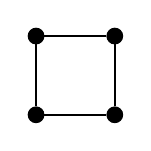
\begin{tikzpicture}
				\node[circle, draw, fill=black, inner sep=2pt] (v1) at (0,0) {};
				\node[circle, draw, fill=black, inner sep=2pt] (v2) at (0,1) {};
				\node[circle, draw, fill=black, inner sep=2pt] (v3) at (1,1) {};
				\node[circle, draw, fill=black, inner sep=2pt] (v4) at (1,0) {};
				
				\draw[thick] (v1) -- (v2);
				\draw[thick] (v1) -- (v4);
				\draw[thick] (v2) -- (v3);
				\draw[thick] (v3) -- (v4);
			\end{tikzpicture}
			\caption{$C_4$}
		\end{subfigure}
		\hfill
		\begin{subfigure}{0.3\textwidth}
			\centering
			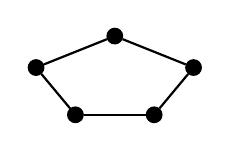
\begin{tikzpicture}
				% Define the vertices using the provided coordinates
				\node[circle, draw, fill=black, inner sep=2pt] (v1) at (0,0) {};
				\node[circle, draw, fill=black, inner sep=2pt] (v2) at (1,0) {};
				\node[circle, draw, fill=black, inner sep=2pt] (v3) at (0.5,1) {};
				\node[circle, draw, fill=black, inner sep=2pt] (v4) at (-0.5,0.6) {};
				\node[circle, draw, fill=black, inner sep=2pt] (v5) at (1.5,0.6) {};
				
				% Draw the edges between all pairs of vertices (complete graph K_5)
				\draw[thick] (v1) -- (v2);
				\draw[thick] (v1) -- (v4);
				\draw[thick] (v2) -- (v5);
				\draw[thick] (v3) -- (v4);
				\draw[thick] (v3) -- (v5);
			\end{tikzpicture}
			\caption{$C_5$}
		\end{subfigure}
	\end{figure}
\end{english}
\newpage
\subsection{البيانات الدولابية \en{Wheels}}
يتم الحصول عليها بإضافة عقدة الى البيانات الدائرية ($n\geq3$) و اضافة سهم من العقدة الجديدة الى كافةالعقد الاخرى. ونرمز لها بــ $W_n$ كما في الشكل التالي
\begin{english}
 	\begin{figure}[H]
 	\centering
 	\begin{subfigure}{0.3\textwidth}
 		\centering
 		\begin{tikzpicture}
 			\node[circle, draw, fill=black, inner sep=2pt] (v1) at (0,0) {};
 			\node[circle, draw, fill=black, inner sep=2pt] (v3) at (0.5,1) {};
 			\node[circle, draw, fill=black, inner sep=2pt] (v4) at (1,0) {};
  			\node[circle, draw, fill=black, inner sep=2pt] (C) at (0.5, 0.33) {};
 			
 			\draw[thick] (v1) -- (v3);
 			\draw[thick] (v1) -- (v4);
 			\draw[thick] (v3) -- (v4);
 			\draw[thick] (C) -- (v1);
 			\draw[thick] (C) -- (v2);
 			\draw[thick] (C) -- (v3); 			 			
 		\end{tikzpicture}
 		\caption{$W_3$}
 	\end{subfigure}
 	\hfill
 	\begin{subfigure}{0.3\textwidth}
 		\centering
 		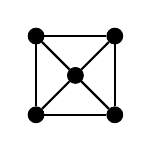
\begin{tikzpicture}
 			\node[circle, draw, fill=black, inner sep=2pt] (v1) at (0,0) {};
 			\node[circle, draw, fill=black, inner sep=2pt] (v2) at (0,1) {};
 			\node[circle, draw, fill=black, inner sep=2pt] (v3) at (1,1) {};
 			\node[circle, draw, fill=black, inner sep=2pt] (v4) at (1,0) {};
  			\node[circle, draw, fill=black, inner sep=2pt] (C) at (0.5, 0.5) {}; 			
 			
 			\draw[thick] (v1) -- (v2);
 			\draw[thick] (v1) -- (v4);
 			\draw[thick] (v2) -- (v3);
 			\draw[thick] (v3) -- (v4);
 			\draw[thick] (C) -- (v1); 			 			
 			\draw[thick] (C) -- (v2); 			 			
 			\draw[thick] (C) -- (v3); 			 			
 			\draw[thick] (C) -- (v4); 			 			
 		\end{tikzpicture}
 		\caption{$W_4$}
 	\end{subfigure}
 	\hfill
 	\begin{subfigure}{0.3\textwidth}
 		\centering
 		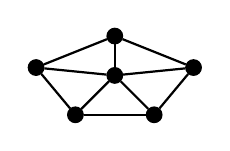
\begin{tikzpicture}
 			% Define the vertices using the provided coordinates
 			\node[circle, draw, fill=black, inner sep=2pt] (v1) at (0,0) {};
 			\node[circle, draw, fill=black, inner sep=2pt] (v2) at (1,0) {};
 			\node[circle, draw, fill=black, inner sep=2pt] (v3) at (0.5,1) {};
 			\node[circle, draw, fill=black, inner sep=2pt] (v4) at (-0.5,0.6) {};
 			\node[circle, draw, fill=black, inner sep=2pt] (v5) at (1.5,0.6) {};
  			\node[circle, draw, fill=black, inner sep=2pt] (C) at (0.5, 0.5) {}; 			
 			
 			% Draw the edges between all pairs of vertices (complete graph K_5)
 			\draw[thick] (v1) -- (v2);
 			\draw[thick] (v1) -- (v4);
 			\draw[thick] (v2) -- (v5);
 			\draw[thick] (v3) -- (v4);
 			\draw[thick] (v3) -- (v5);
 			\draw[thick] (C) -- (v1); 			 			
 			\draw[thick] (C) -- (v2); 			 			
 			\draw[thick] (C) -- (v3); 			 			
 			\draw[thick] (C) -- (v4); 			 			
 			\draw[thick] (C) -- (v5); 			 			
 		\end{tikzpicture}
 		\caption{$W_5$}
 	\end{subfigure}
 \end{figure}
 \end{english}
 
 \section{تمثيل البيانات \en{Representing Graphs}}
 
 \subsection{مصفوفة الجوار \en{Adjacency Matrix}}
 ليكن لدينا البيان غير الموجه $G= (G, V)$ المكون من مجموعة العقد 
 $V = \{v_1, \dots, v_n\}$
نعرف مصفوفة الجوار للبيان $G$ على انها المصفوفة المربعة $A = [a_{ij}]$ ذات البعد $n\times n$ المعرفة على النحو التالي
$a_{ij}$ يساوي عدد الاسهم التي تربط العقدة $v_i$ بالعقدة $v_j$.
 
\noindent
\textbf{مثال}\\
اوجد مصفوفة الجوار للبيان التالي
\begin{figure}[H]
	\centering
	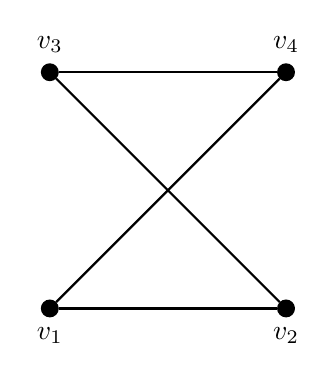
\begin{tikzpicture}[thick]
		\node[fill=black, circle, draw, inner sep=2pt, label={below: $v_1$}] (v1) at (0,0) {};
		\node[fill=black, circle, draw, inner sep=2pt, label={below: $v_2$}] (v2) at (3,0) {};
		\node[fill=black, circle, draw, inner sep=2pt, label={above: $v_3$}] (v3) at (0,3) {};
		\node[fill=black, circle, draw, inner sep=2pt, label={above: $v_4$}] (v4) at (3,3) {};
		
		\draw (v1) -- (v2);
		\draw (v1) -- (v4);
		\draw (v3) -- (v2);
		\draw (v3) -- (v4);
	\end{tikzpicture}
\end{figure}
\noindent
\textbf{الحل}
\begin{english}
	\[
\begin{bNiceMatrix}[first-row,first-col]
	&v_1&v_2&v_3&v_4\\
	v_1 & 0 & 1 & 1 & 0\\
	v_2 & 1 & 0 & 0 & 1\\
	v_3& 1 & 0 & 0 & 1\\
	v_4& 0 & 1 & 1 & 0
\end{bNiceMatrix}
\]
\end{english}
\newpage
\noindent
\textbf{مثال}\\
\noindent
اوجد مصفوفة الجوار للبيان التالي
\begin{figure}[H]
	\centering
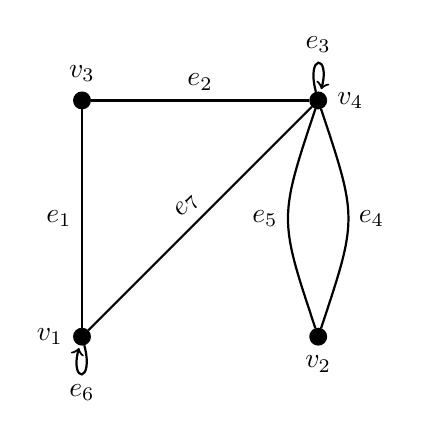
\begin{tikzpicture}[thick]
			\node[fill=black, circle, draw, inner sep=2pt, label={left: $v_1$}] (v1) at (0,0) {};
\node[fill=black, circle, draw, inner sep=2pt, label={below: $v_2$}] (v2) at (3,0) {};
\node[fill=black, circle, draw, inner sep=2pt, label={above: $v_3$}] (v3) at (0,3) {};
\node[fill=black, circle, draw, inner sep=2pt, label={right: $v_4$}] (v4) at (3,3) {};

	\path (v1) edge node[midway, left] {$e_1$} (v3);
	\path (v3) edge node[midway, above] {$e_2$} (v4);
	\path (v1) edge node[midway, above, sloped] {$e_7$} (v4);
	\path (v4) edge [loop above] node[midway, above] {$e_3$} (v4);
	\path (v1) edge [loop below] node[midway, below] {$e_6$} (v1);
	\draw[thick] (v2) .. controls (3.5,1.5) .. (v4) node[midway, right]{$e_4$};
	\draw[thick] (v2) .. controls (2.5,1.5) .. (v4) node[midway, left]{$e_5$};
\end{tikzpicture}
\end{figure}
\noindent
\textbf{الحل}
\begin{english}
	\[
	\begin{bNiceMatrix}[first-row,first-col]
		&v_1&v_2&v_3&v_4\\
		v_1 & 0 & 1 & 0& 0\\
		v_2 & 1 & 1 & 2 & 1\\
		v_3& 0 & 2 & 0 & 0\\
		v_4& 1 & 1 & 0 & 1
	\end{bNiceMatrix}
	\]
\end{english}

\subsection{مصفوفة الورود \en{Incidence Matrix}}
ليكن لدينا البيان غير الموجه $G= (G, V)$ المكون من مجموعة العقد 
$V = \{ v_1, v_2, \dots, v_n\}$
و مجموعة الاسهم
$E = \{e_1, e_2, \dots, e_m\}$
نعرف مصفوفة الورود للبيان $G$ على انها المصفوفة $M = [m_{ij}]$ ذات البعد $n\times m$ على النحو التالي
\[
m_{ij} =
\begin{cases}
	1 & \text{عندما السهم $e_j$ يصل العقدة $v_i$} \\
	0 & \text{otherwise}
\end{cases}
\]
\newpage
\noindent
\textbf{مثال}\\
\noindent
اوجد مصفوفة الورود للبيان التالي
\begin{figure}[H]
	\centering
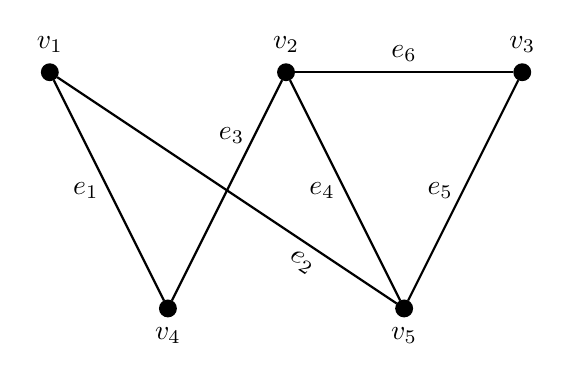
\begin{tikzpicture}[thick]
		\node[fill=black, circle, draw, inner sep=2pt, label={above: $v_1$}] (v1) at (0,0) {};
	\node[fill=black, circle, draw, inner sep=2pt, label={above: $v_2$}] (v2) at (3,0) {};
	\node[fill=black, circle, draw, inner sep=2pt, label={above: $v_3$}] (v3) at (6,0) {};
	\node[fill=black, circle, draw, inner sep=2pt, label={below: $v_4$}] (v4) at (1.5,-3) {};
	\node[fill=black, circle, draw, inner sep=2pt, label={below: $v_5$}] (v5) at (4.5,-3) {};
	
		\path (v1) edge node[midway, left] {$e_1$} (v4);
		\path (v1) edge node[pos=0.75, sloped, below] {$e_2$} (v5);
		\path (v2) edge node[pos=0.25, left] {$e_3$} (v4);
		\path (v2) edge node[midway, left] {$e_4$} (v5);
		\path (v2) edge node[midway, above] {$e_6$} (v3);
		\path (v3) edge node[midway, left] {$e_5$} (v5);
\end{tikzpicture}
\end{figure}
\noindent
\textbf{الحل}
\begin{english}
	\[
	\begin{bNiceMatrix}[first-row,first-col]
		& e_1 & e_2 & e_3 & e_4 & e_5 & e_6 \\
		v_1 & 1 & 1 & 0 & 0 & 0 & 0 \\
		v_2 & 0 & 0 & 1 & 1 & 0 & 1 \\
		v_3 & 0 & 0 & 0 & 0 & 1 & 1 \\
		v_4 & 1 & 0 & 1 & 0 & 0 & 0 \\
		v_5 & 0 & 1 & 0 & 1 & 1 & 0
	\end{bNiceMatrix}
	\]
\end{english}

\begin{example}
	اوجد البيان الموجه الذي مصفوفة جواره 
\[
\begin{bmatrix}
	0&1&1&0\\
	1&1&0&2\\
	0&0&1&1\\
	2&1&0&0
\end{bmatrix}
\]
\end{example}

\noindent
\textbf{الحل}\\
\noindent
ليكن $G$ البيان الموافق لمصفوفة الجوار اعلاه. وليكن $v_1, v_2, v_3, v_4$ مجموعة عقد البيان $G$
	\setLR
\[
\begin{bNiceMatrix}[first-row,first-col]
	&v_1&v_2&v_3&v_4\\
	v_1 & 0 & 1 & 1& 0\\
	v_2 & 1 & 1 & 0 & 2\\
	v_3& 0 & 0 & 1 & 1\\
	v_4& 2 & 1 & 0 & 0
\end{bNiceMatrix}
\]\setRL
وبالتالي يكون البيان الموجه الموافق للمصفوفة هو التالي

\begin{figure}[H]
	\centering
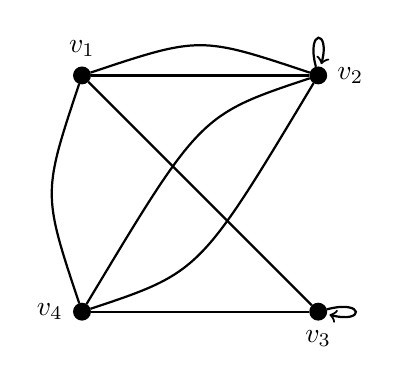
\begin{tikzpicture}[thick]
	\node[fill=black, circle, draw, inner sep=2pt, label={left: $v_4$}] (v4) at (0,0) {};
	\node[fill=black, circle, draw, inner sep=2pt, label={below: $v_3$}] (v3) at (3,0) {};
	\node[fill=black, circle, draw, inner sep=2pt, label={above: $v_1$}] (v1) at (0,3) {};
	\node[fill=black, circle, draw, inner sep=2pt, label={right: $v_2$}] (v2) at (3,3) {};
	
	\draw (v1) -- (v2);
	\draw (v3) -- (v4);
	\draw (v1) -- (v3);
	\path (v3) edge [loop right] (v3);
	\path (v2) edge [loop above] (v2);
	\draw (v1) .. controls (1.5, 3.5) .. (v2);
	\draw (v1) .. controls (-0.5, 1.5) .. (v4);
	\draw (v4) .. controls (1.5, 2.5) .. (v2);
	\draw (v4) .. controls (1.5, 0.5) .. (v2);
\end{tikzpicture}
\end{figure}

\section{الترابطية Connectivity}
\subsection*{الترابطية في البيانات غير الموجهة}
نعرف المسار Path بطول $n\geq 0$ من العقدة $u$ الى العقدة $v$ ضمن بيان غير موجه $G$ على انه سلسلة مكونة من $n$ من الاسهم $e_1,\dots,e_n$ من البيان $G$ وحيث ان 
\[
\{x_0=u, x_1\}=e_0, \{x_1,x_2\} = e_2,\dots, \{x_{n-1}, x_{n}=v\}=e_n
\]
عندما يكون المسار بسيط نرمز للمسار بسلسلة العقد $x_1,x_2,\dots,x_n$ ونسمي مساراً على انه دائرة اذا كان يبدأ وينتهي بنفس العقدة ، اي ان $u=v$ كما ندعوا مساراً بسيطاً اذا كان لا يحوي على نفس السهم اكثر من مرة ولحدة.

\begin{example}
	ليكن البيان البسيط التالي
	\begin{figure}[H]
		\centering
		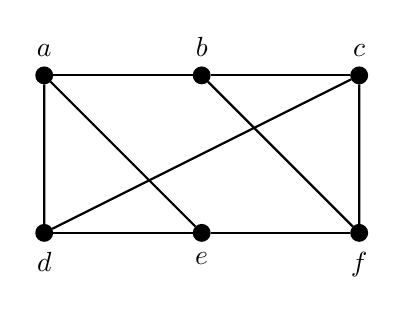
\begin{tikzpicture}[thick]
	\node[fill=black, circle, draw, inner sep=2pt, label={above: $a$}] (a) at (0,0) {};
	\node[fill=black, circle, draw, inner sep=2pt, label={above: $b$}] (b) at (2,0) {};
	\node[fill=black, circle, draw, inner sep=2pt, label={above: $c$}] (c) at (4,0) {};
	\node[fill=black, circle, draw, inner sep=2pt, label={below: $d$}] (d) at (0,-2) {};
	\node[fill=black, circle, draw, inner sep=2pt, label={below: $e$}] (e) at (2,-2) {};
	\node[fill=black, circle, draw, inner sep=2pt, label={below: $f$}] (f) at (4,-2) {};
	
	\draw (a) -- (b) -- (c);
	\draw (d) -- (a) -- (e);
	\draw (b) -- (f);
	\draw (f) -- (c)-- (d);
	\draw (d) -- (e) -- (f);
		\end{tikzpicture}
	\end{figure}
	\noindent
	$a, b, c,d,e,f$ عبارة عن مسار بسيط طوله 4.\\
	$a, c , e, d$ ليست مساراً.\\
	$b, c, f, e, b$ عبارة عن دائرة طولها 4.\\
	$a, b, e, d, a, b$ عبارة عن مسار طوله 4 ولكنه غير بسيط لانه يحوي السهم $\{a, b\}$ مرتين.
\end{example}

\begin{definition}
	نقول عن بيان غير موجه على انه مترابط connected اذا وجد مسار بين كل زوج من عقد البيان المختلفة.
\end{definition}

\begin{theorem}
	يوجد مسار بسيط بين اي عقدتين مختلفتين في بيان مترابط غير موجه.
\end{theorem}

\begin{example}
ليكن لدينا البيانين التاليين
	\begin{figure}[H]
		\centering
		\begin{subfigure}{0.3\textwidth}
			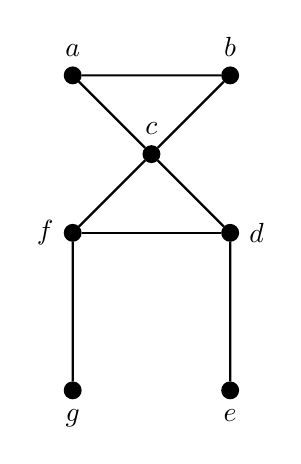
\begin{tikzpicture}[thick]
					\node[fill=black, circle, draw, inner sep=2pt, label={above: $a$}] (a) at (0,0) {};
				\node[fill=black, circle, draw, inner sep=2pt, label={above: $b$}] (b) at (2,0) {};
				\node[fill=black, circle, draw, inner sep=2pt, label={above: $c$}] (c) at (1,-1) {};
				\node[fill=black, circle, draw, inner sep=2pt, label={right: $d$}] (d) at (2,-2) {};
				\node[fill=black, circle, draw, inner sep=2pt, label={below: $e$}] (e) at (2,-4) {};
				\node[fill=black, circle, draw, inner sep=2pt, label={left: $f$}] (f) at (0,-2) {};
				\node[fill=black, circle, draw, inner sep=2pt, label={below: $g$}] (g) at (0,-4) {};
				
				\draw (e) -- (d) -- (c) -- (a) -- (b);
				\draw (g)--(f)--(c)--(b);
				\draw (f)--(d);
			\end{tikzpicture}
			\caption{$G_1$}
		\end{subfigure}
		\begin{subfigure}{0.3\textwidth}
			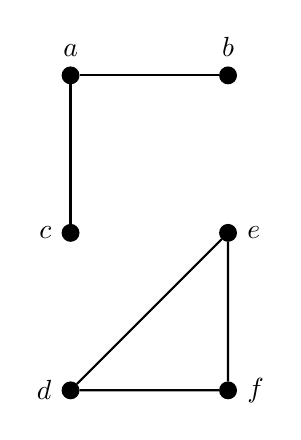
\begin{tikzpicture}[thick]
					\node[fill=black, circle, draw, inner sep=2pt, label={above: $a$}] (a) at (0,0) {};
				\node[fill=black, circle, draw, inner sep=2pt, label={above: $b$}] (b) at (2,0) {};
				\node[fill=black, circle, draw, inner sep=2pt, label={left: $c$}] (c) at (0,-2) {};
				\node[fill=black, circle, draw, inner sep=2pt, label={left: $d$}] (d) at (0,-4) {};
				\node[fill=black, circle, draw, inner sep=2pt, label={right: $e$}] (e) at (2,-2) {};
				\node[fill=black, circle, draw, inner sep=2pt, label={right: $f$}] (f) at (2,-4) {};
				
				\draw (c)--(a)--(b);
				\draw (d)--(e)--(f)--(d);
			\end{tikzpicture}
			\caption{$G_2$}
		\end{subfigure}
	\end{figure}
	\noindent
	من الواضح ان البيان $G_1$ مترابط لانه يوجد بين  اي زوج من العقد المختلفة مسار. بينما البيان $G_2$ غير مترابط لانه لا يوجد مسار بين العقدتين $a, d$
\end{example}

\subsection*{عدد المسارات بين العقد \LR{Counting paths betwwn vertices}}

\begin{theorem}
	ليكن $G$ بيان مصفوفة جواره $A$ بالنسبة لمجموعة العقد $v_1, v_2, \dots, v_n$ التي يتكون منها ، ان عدد المسارات المختلفة بطول $r$ من العقدة $v_i$ الى العقدة $v_j$ يساوي العنصر $(i,j)$ من المصفوفة $A^r$.
\end{theorem}
\newpage
\begin{example}
	ما هو عدد المسارت بطول 4 من العقدة $a$ الى العقدة $b$ في البيان البسيط  التالي
	\begin{figure}[H]
		\centering
		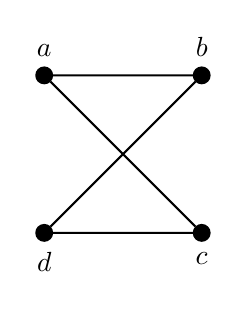
\begin{tikzpicture}[thick]
			\node[fill=black, circle, draw, inner sep=2pt, label={above: $a$}] (a) at (0,0) {};
\node[fill=black, circle, draw, inner sep=2pt, label={above: $b$}] (b) at (2,0) {};
\node[fill=black, circle, draw, inner sep=2pt, label={below: $c$}] (c) at (2,-2) {};
\node[fill=black, circle, draw, inner sep=2pt, label={below: $d$}] (d) at (0,-2) {};

\draw (a) -- (b) -- (d) -- (c) -- (a);
		\end{tikzpicture}
	\end{figure}
\end{example}
\begin{solution}
	ان مصفوفة الجوار للبيان بالنسبة للعقد $a, b, c, d$ هي
	\[
	A=\begin{bmatrix}
		0&1&1&0\\
		1&0&0&1\\
		1&0&0&1\\
		0&1&1&0
	\end{bmatrix}
	\]
	بالتالي فان عدد المسارت بطول 4 من العقدة $a$ الى العقدة $d$ هو العنصر $(1, 4) = 8$ من المصفوفة $A^4$
	\[
	A^4=
	\begin{bmatrix}
		0&8&8&0\\
		8&0&0&8\\
		8&0&0&8\\
		0&8&8&0
	\end{bmatrix}
	\]
	المسارات الثمانية هي التالية 
	\[
	a, b, a, b, d \to a, b, a, c,d \to a,b,d,b,d\to a,b,d,c,d
	\]
	\[
	a,c,a,b,d \to a,c,a,c,d \to a,c,d,b,d \to a,c,d,c,d
	\]
\end{solution}